\documentclass[11pt,a4paper,oneside]{article}

\usepackage[utf8]{vietnam}
\usepackage[english]{babel}
\usepackage{freecontest}
\usepackage{verbatim}
\usepackage{graphicx}
\usepackage{wrapfig}
\usepackage{tabularx}

\header{\LARGE Free Contest 120}

\begin{document}

\problemtitle{CAROM}
\\
Đậu là một cậu bé có ước mơ trở thành cơ thủ carom chuyên nghiệp. Để thực hiện ước mơ đó, cậu dành hàng giờ trên bàn carom đã cũ để rèn luyện các kĩ thuật đánh khác nhau. Chiếc bàn carom của Đậu có thể được coi là một hình chữ nhật kích thước $h \times w$ trên mặt phẳng tọa độ $Oxy$ với 4 đỉnh có tọa độ $(0;0), (w;0), (w;h),$ và $(h;0)$. Do chiếc bàn đã cũ nên trên mặt bàn có một lỗ thủng hình đa giác không tự cắt có các cạnh song song với cạnh bàn. Trong tuần tới, Đậu sẽ luyện tập duy nhất một kĩ thuật là cú đánh hướng đông bắc sao cho bi cái chuyển động đều. Đậu cần xác định thời điểm và vị trí rơi xuống lỗ thủng của bi cái để tiện cho việc thu thập bi trong lúc luyện tập. Hãy viết chương trình giúp Đậu làm việc này. \\\\
Để đơn giản hóa bài toán, lỗ thủng của chiếc bàn sẽ có các đỉnh là tọa độ nguyên  và không có cạnh nào có điểm chung với cạnh bàn. Ngoài ra, Đậu cũng sẽ đặt bi cái ở các điểm có tọa độ nguyên, và đánh bi sao cho bi cái bắt đầu chuyển động đều với vận tốc $(1;1)$ (tức cứ mỗi giây, tọa độ $x$ và $y$ của bi cái tăng một đơn vị). Do bi cái khá nhỏ so với bàn carom, ta cũng có thể coi bi cái là một chất điểm. Điểm khó của bài toán là khi bi cái va chạm với cạnh bàn hoặc góc bàn, bi cái sẽ đổi hướng như trong hình dưới đây:
\begin{center}
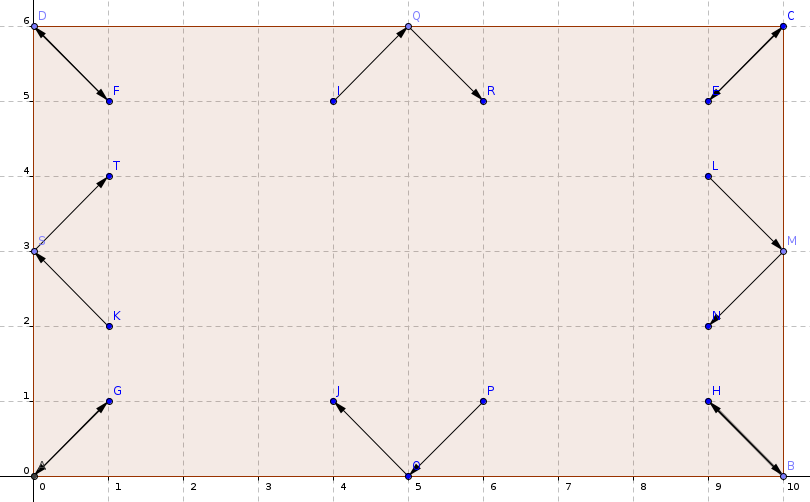
\includegraphics[scale=0.5]{carom.png}
\end{center}
Cụ thể hơn, giả sử vận tốc của bi cái đang là $(v_x;v_y)$:
\begin{itemize}
\item Nếu bi cái chạm vào một cạnh song song với trục $Ox$, vận tốc của bi cái sẽ chuyển thành $(v_x;-v_y)$.
\item Nếu bi cái chạm vào một cạnh song song với trục $Oy$, vận tốc của bi cái sẽ chuyển thành $(-v_x;v_y)$
\item Nếu bi cái chạm vào góc bàn (hai cạnh cùng một lúc), vận tốc của bi cái sẽ chuyển thành $(-v_x;-v_y)$.
\end{itemize}
\heading{Dữ liệu}
\begin{itemize}
\item Dòng đầu tiên gồm hai số nguyên dương $w, h$ ($1 \leq w,h \leq 5 \times 10^8$) mô tả kích thước của bàn carom.
\item Dòng thứ hai gồm một số nguyên dương $n$ ($4 \leq n \leq 1000$) mô tả số đỉnh của lỗ thủng trên bàn carom.
\item $n$ dòng tiếp theo, mỗi dòng gồm hai số nguyên dương $x_i, y_i$ ($1 \leq x_i \leq w-1, 1 \leq y_i \leq h-1$) là các đỉnh của lỗ thủng trên bàn carom. Các đỉnh trong dữ liệu vào được cho theo thứ tự thuận chiều kim đồng hồ hoặc ngược chiều kim đồng hồ. Không có hai đỉnh nào trùng nhau, cũng như không có ba đỉnh \textbf{liên tiếp} thẳng hàng. 
\item Dòng tiếp theo chứa một số nguyên dương $q$ ($1 \leq q \leq 100$) là số lần Đậu luyện tập cú đánh của mình.
\item $q$ dòng tiếp theo, dòng thứ $i$ gồm hai số nguyên dương $x_s, y_s$ ($1 \leq x_s \leq w-1, 1 \leq y_s \leq h-1$) là tọa độ điểm Đậu đặt bi cái trong lần luyện tập thứ $i$ của mình. 
\end{itemize}
\heading{Kết quả}
Với mỗi lần luyện tập của Đậu:
\begin{itemize}
\item Nếu bi cái không bao giờ rơi xuống lỗ thủng trên mặt bàn, in một dòng chứa \texttt{-1}.
\item Nếu bi cái sẽ rơi xuống lỗ thủng trên mặt bàn, in một dòng chứa ba số nguyên $t, x_f, y_f$ lần lượt là thời điểm bi cái rơi xuống lỗ và tọa độ $(x_f; y_f)$ của vị trí của bi cái khi rơi xuống lỗ. Tọa độ $(x_f; y_f)$ phải là một điểm nằm trên chu vi của lỗ thủng.
\end{itemize} 
\heading{Ví dụ}
\begin{example}
\exmp{%
4 4
4
1 1
1 2
2 2
2 1
1
1 3 \\
}{%
6 1 1
}%
\end{example}
\heading{Giải thích}
\begin{center}
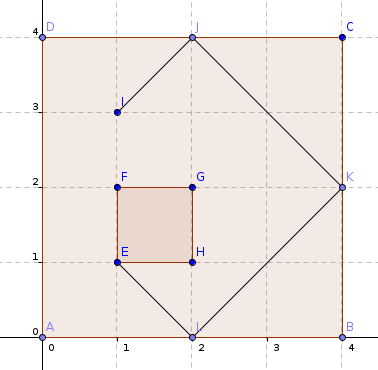
\includegraphics[scale=0.5]{carom2.png} 
\end{center}
Ở ví dụ đầu tiên, hình $ABCD$ là mặt bàn carom, hình $EFGH$ là lỗ thủng trên bàn carom, và điểm $I$ là điểm mà Đậu đặt bi cái. Bi cái di chuyển theo đường gấp khúc $IJKLE$, và chạm vào điểm $E$ của lỗ thủng sau 6 giây di chuyển.
\end{document}